\documentclass[12pt, titlepage]{article}

\usepackage{amssymb}
\usepackage{amstext}
\usepackage{amsthm}
\usepackage{amsmath}
\usepackage{enumerate}
\usepackage{enumitem}
\usepackage{fancyhdr}
\usepackage[margin=1in]{geometry}
\usepackage{graphicx}
\usepackage{extarrows}
\usepackage{setspace}
\usepackage{hhline}
\usepackage{lscape}
\usepackage{multirow}

\usepackage{booktabs}
\usepackage{tabularx}
\usepackage{float}
\usepackage{hyperref}
\hypersetup{
    colorlinks,
    citecolor=black,
    filecolor=black,
    linkcolor=black,
    urlcolor=blue
}
\usepackage[round]{natbib}
\usepackage{titlesec}
\usepackage{placeins}
\usepackage{graphicx}
\usepackage{xkeyval}
\usepackage[dvipsnames]{xcolor} % for different colour comments
\usepackage{tabto}
\usepackage{mdframed}
\usepackage{lscape}
\usepackage{multirow}


\title{SE 3XA3: Test Report\\Ultimate Calculator}

\author{Group 15 L01
		\\ Jarod Rankin, rankij5
		\\ Mathew Petronilho, petronim
		\\ Logan Brown, brownl33
		\\ Syed Bokhari, bokhars
}

\date{\today}


%\input{../Comments}

\begin{document}

\maketitle

\pagenumbering{roman}
\tableofcontents
\listoftables
\listoffigures

\begin{table}[bp]
\caption{\bf Revision History}
\begin{tabularx}{\textwidth}{p{3cm}p{2cm}X}
\toprule {\bf Date} & {\bf Version} & {\bf Notes}\\
\midrule
April 5 2022 & 1.0 & FR and NFR Evaluation\\
April 7 2022 & 1.1 & Rest of document complete\\
\bottomrule
\end{tabularx}
\end{table}

\newpage

\pagenumbering{arabic}

This document outlines the results of all the testing done for the Ultimate Calculator, as stated in the test plan.

\section{Functional Requirements Evaluation}
\subsection{Calculation Testing}
\begin{enumerate}

\item[Test:]{FR-C-T1\\}

\textbf{Description:} Test to ensure all operation section windows open properly, they each have a way to calculate an output, and can calculate the correct output synchronously along with the other windows

\textbf{Type:} Functional, Dynamic, Manual
					
\textbf{Initial State:} Operation section windows are open
					
\textbf{Input:} Press of the calculate button on each window
					
\textbf{Output:} The operation answer in the respective operation section window

\textbf{Expected:} The correct output of the answer should be visible in the output text box when the calculate button is pressed. Calculations can be run synchronously

\textbf{Result:} \textcolor{Green}{Pass}


\item[Test:]{FR-C-T2\\}

\textbf{Description:} Test to determine if appropriate error message is returned after mathematical operations with undefined outputs

\textbf{Type:} Functional, Dynamic, Manual
					
\textbf{Initial State:} Operation section window is open 
					
\textbf{Input:} Numbers that will cause undefined outputs
					
\textbf{Output:} Error message

\textbf{Expected:} Application should remain working and error message should be displayed

\textbf{Result:} \textcolor{Green}{Pass}

\item[Test:]{FR-C-T3\\}

\textbf{Description:} Test to determine if calculator outputs are mathematically correct

\textbf{Type:} Unit, Dynamic, Automated
					
\textbf{Initial State:} Application is running
					
\textbf{Input:} Valid arbitrary inputs
					
\textbf{Output:} Correct calculation

\textbf{Expected:} All operations implemented by the calculator should return mathematically correct results

\textbf{Result:} \textcolor{Green}{Pass}


\end{enumerate}

\subsection{User Interface Testing}

\begin{enumerate}

\item[Test:]{FR-UI-T1\\}

\textbf{Description:} Test to determine if application starts at main menu and that all operation types are visible from there

\textbf{Type:} Functional, Dynamic, Manual
					
\textbf{Initial State:} An empty command line terminal
					
\textbf{Input:} Initialization of the Ultimate Calculator application through the command line
					
\textbf{Output:} A main menu window for the application

\textbf{Expected:} The main menu along with the operation types of conversions, algebra, stocks, health, GPA, geometry, and binary should all be visible

\textbf{Result:} \textcolor{Green}{Pass}

\item[Test:]{FR-UI-T2\\}

\textbf{Description:} Test to determine if the minimum amount of operation types are present

\textbf{Type:} Functional, Dynamic, Manual
					
\textbf{Initial State:} Main menu for the application has been initialized
					
\textbf{Input:} Selection of all operation types
					
\textbf{Output:} The operation type windows

\textbf{Expected:} The amount of operation types present in the system is more than \hyperref[sec:sp]{MIN\_UNIQUE\_OP}

\textbf{Result:} In total there are 7 unique operation types, which is more than \hyperref[sec:sp]{MIN\_UNIQUE\_OP}\\ \textcolor{Green}{Pass}

\item[Test:]{FR-UI-T3\\}

\textbf{Description:} Test to determine if the minimum amount of operation types are present and that they all open with empty inputs

\textbf{Type:} Functional, Dynamic, Manual
					
\textbf{Initial State:} Operation type windows are open
					
\textbf{Input:} Selection of all operations belonging to a specific operation type
					
\textbf{Output:} The operation sections

\textbf{Expected:} The amount of operation sections present for each operation type is more than \hyperref[sec:sp]{MIN\_OP\_SECTION}. Inputs are empty upon opening of each operation section

\textbf{Result:} Each operation type has the required amount of operation sections and they all open with empty inputs\\ \textcolor{Green}{Pass}

\item[Test:]{FR-UI-T4\\}

\textbf{Description:} Test to determine if each operation window has the total number of inputs be equal to or greater than \hyperref[sec:sp]{MIN\_INPUT}, and ensure that each input field allows the user to properly input values

\textbf{Type:} Functional, Dynamic, Manual
					
\textbf{Initial State:} Operation type windows are open
					
\textbf{Input:} Selection of all operation section windows
					
\textbf{Output:} The operation sections

\textbf{Expected:} Each input field in each operation window should be visually populated with a number

\textbf{Result:} \textcolor{Green}{Pass}

\item[Test:]{FR-UI-T5\\}

\textbf{Description:} Test to determine if error message is displayed for invalid inputs

\textbf{Type:} Functional, Dynamic, Manual
					
\textbf{Initial State:} Operation section window is open 
					
\textbf{Input:} Non-valid input type
					
\textbf{Output:} Warning

\textbf{Expected:} Application should not crash upon entering invalid inputs, and should display a message to tell the user an error occurred

\textbf{Result:} Every operation section outputs appropriate error message with invalid input\\
\textcolor{Green}{Pass}


\item[Test:]{FR-UI-T6\\}

\textbf{Description:} Test to determine if error message is displayed after attempting to calculate with empty inputs

\textbf{Type:} Functional, Dynamic, Manual
					
\textbf{Initial State:} Operation section window is open
					
\textbf{Input:} Empty inputs

\textbf{Output:} Warning

\textbf{Expected:} Application should not crash upon entering no inputs, and should display a message to tell the user an error occurred

\textbf{Result:} \textcolor{Green}{Pass}


\item[Test:]{FR-UI-T7\\}

\textbf{Description:} Test to determine if an output is always displayed with valid arbitrary inputs

\textbf{Type:} Functional, Dynamic, Manual
					
\textbf{Initial State:} Operation section window is open
					
\textbf{Input:} Valid arbitrary inputs
					
\textbf{Output:} Display of output

\textbf{Expected:} Application should display the result of the calculation to the user interface

\textbf{Result:} \textcolor{Green}{Pass}
					

\item[Test:]{FR-UI-T8\\}

\textbf{Description:} Test to verify clear button works on applicable operation sections

\textbf{Type:} Functional, Dynamic, Manual
					
\textbf{Initial State:} Operation section window is open
					
\textbf{Input:} Clear button
					
\textbf{Output:} Empty text boxes

\textbf{Expected:} Application should clear any text boxes of their current text

\textbf{Result:} \textcolor{Green}{Pass}

\item[Test:]{FR-UI-T9\\}

\textbf{Description:} Test to determine if each operation window has a close button and the window closes once the button is clicked

\textbf{Type:} Functional, Dynamic, Manual
					
\textbf{Initial State:} Operation windows are open
					
\textbf{Input:} Selection of the close button on the operation window
					
\textbf{Output:} Operation type window closes

\textbf{Expected:} The operation type windows will close once the close button is clicked

\textbf{Result:} \textcolor{Green}{Pass}

\item[Test:]{FR-UI-T10\\}

\textbf{Description:} Test to determine if each window has a close button and if the main calculator window prompts the user with a question confirming their choice to close the program. All windows should close when the main menu window is closed 

\textbf{Type:} Functional, Dynamic, Manual
					
\textbf{Initial State:} Operation type and main menu windows are open
					
\textbf{Input:} Selection of the close button on the main menu window 
					
\textbf{Output:} Operation type window closes

\textbf{Expected:} The operation type windows and the main calculator windows will close once the close button is clicked from the main menu window and the dialog is confirmed

\textbf{Result:} \textcolor{Green}{Pass}

\end{enumerate}

\section{Nonfunctional Requirements Evaluation}

\subsection{Look and Feel Testing}
\begin{enumerate}

\item[Test:]{NFR-LF-T1\\}

\textbf{Description:} Tests that the main menu GUI is similar in appearance to a standard calculator

\textbf{Type:} Static, Manual
					
\textbf{Tester(s):} Survey participants
					
\textbf{Pass:} Average \hyperref[sec:surveyR]{survey} score of at least \hyperref[sec:sp]{SURVEY\_SCORE}\% for question 1
					
\textbf{Result:} \textcolor{Green}{Pass}

\item[Test:]{NFR-LF-T2\\}

\textbf{Description:} Tests that the GUIs of the application all have a coherent design

\textbf{Type:} Static, Manual
					
\textbf{Tester(s):} Testing team and survey participants
					
\textbf{Pass:} All font styles, font sizes, colours, and buttons used in the application are consistent and an average \hyperref[sec:surveyR]{survey} score of at least \hyperref[sec:sp]{SURVEY\_SCORE}\% for question 2
					
\textbf{Result:} \textcolor{Green}{Pass}

\end{enumerate}

		
\subsection{Usability Testing}
\begin{enumerate}

\item[Test:]{NFR-U-T1\\}

\textbf{Description:} Tests that all the navigational buttons open up the correct windows and that all operation sections can be reached easily

\textbf{Type:} Dynamic, Manual
					
\textbf{Tester(s):} Testing team
					
\textbf{Pass:} Navigational buttons open their corresponding windows and all operation sections can be reached within \hyperref[sec:sp]{MAX\_NAVIGATION\_CLICKS} mouse clicks from the main menu
					
\textbf{Result:} \textcolor{Green}{Pass}

\item[Test:]{NFR-U-T2\\}

\textbf{Description:} Tests that the navigational buttons on the application are descriptive and contain icons that allow the user to seamlessly transition from one menu to another

\textbf{Type:} Dynamic, Manual
					
\textbf{Tester(s):} Testing team
					
\textbf{Pass:} \hyperref[sec:surveyR]{Results} from the usability survey determine that users found the buttons descriptive and that navigating through the application was easy
					
\textbf{Result:} \textcolor{Green}{Pass}


\end{enumerate}

\subsection{Performance Testing}
\begin{enumerate}
    
\item[Test:]{NFR-P-T1\\}

\textbf{Description:} Tests that when the application opens each window the window will open in equal to or less than the \hyperref[sec:sp]{MAX\_RESPONSE\_TIME}

\textbf{Type:} Functional, Dynamic, Manual

\textbf{Tester(s):} Testing team

\textbf{Pass:} Each window is opened in less than the \hyperref[sec:sp]{MAX\_RESPONSE\_TIME}
					
\textbf{Result:} \textcolor{Green}{Pass}

\item[Test:]{NFR-P-T2\\}

\textbf{Description:} Tests that when the application opens each operation window the application will compute an answer for each operation type equal to or less than the \hyperref[sec:sp]{MAX\_RESPONSE\_TIME}

\textbf{Type:} Functional, Dynamic, Manual

\textbf{Tester(s):} Testing team

\textbf{Pass:} Each operation is completed in less than the \hyperref[sec:sp]{MAX\_RESPONSE\_TIME}
					
\textbf{Result:} \textcolor{Green}{Pass}

\item[Test:]{NFR-P-T3\\}

\textbf{Description:} Tests that outputs to calculations give a maximum number of significant digits

\textbf{Type:} Functional, Dynamic, Manual

\textbf{Tester(s):} Testing Team

\textbf{Pass:} Arbitrary valid input gives outputs with \hyperref[sec:sp]{MAX\_SIG\_FIGS} amount of significant digits
					
\textbf{Result:} \textcolor{Green}{Pass}

\end{enumerate}

\subsection{Operational and Environmental Testing}
\begin{enumerate}
    
\item[Test:]{NFR-OE-T1\\}

\textbf{Description:} Tests that the application works without an internet connection

\textbf{Type:} Functional, Dynamic, Manual

\textbf{Tester(s):} Testing team

\textbf{Pass:} Application starts while disconnected from internet
					
\textbf{Result:} \textcolor{Green}{Pass}


\end{enumerate}

\subsection{Maintainability and Support Requirements}

\begin{enumerate}
\item[Test:]{NFR-MS-T1\\}

\textbf{Description:} Tests that the application is an open source software where anyone can submit bugs and issues

\textbf{Type:} Structural, Static, Manual
					
\textbf{Tester(s):} Testing team
					
\textbf{Pass:} The code base is accessible via GitHub or GitLab and the tester is able to create an open issue and track the status of the changes.  
					
\textbf{Result:} \textcolor{Green}{Pass}

\item[Test:]{NFR-MS-T2\\}

\textbf{Description:} Tests that the system allows new operations to be added

\textbf{Type:} Structural, Static, Manual
					
\textbf{Tester(s):} Testing team
					
\textbf{Pass:} The code base is viewed and the code is modular exhibits low coupling and high cohesion
					
\textbf{Result:} \textcolor{Green}{Pass}

\end{enumerate}


\subsection{Survey Results}
\label{sec:surveyR}

As mentioned in the test plan, we conducted a \hyperref[sec:survey]{survey} to evaluate the usability and appearance of the calculator. We surveyed 10 people, including fellow students and family members. The results can be seen in \hyperref[calc]{Figure 1}.

\begin{figure}[H]
    \centering
    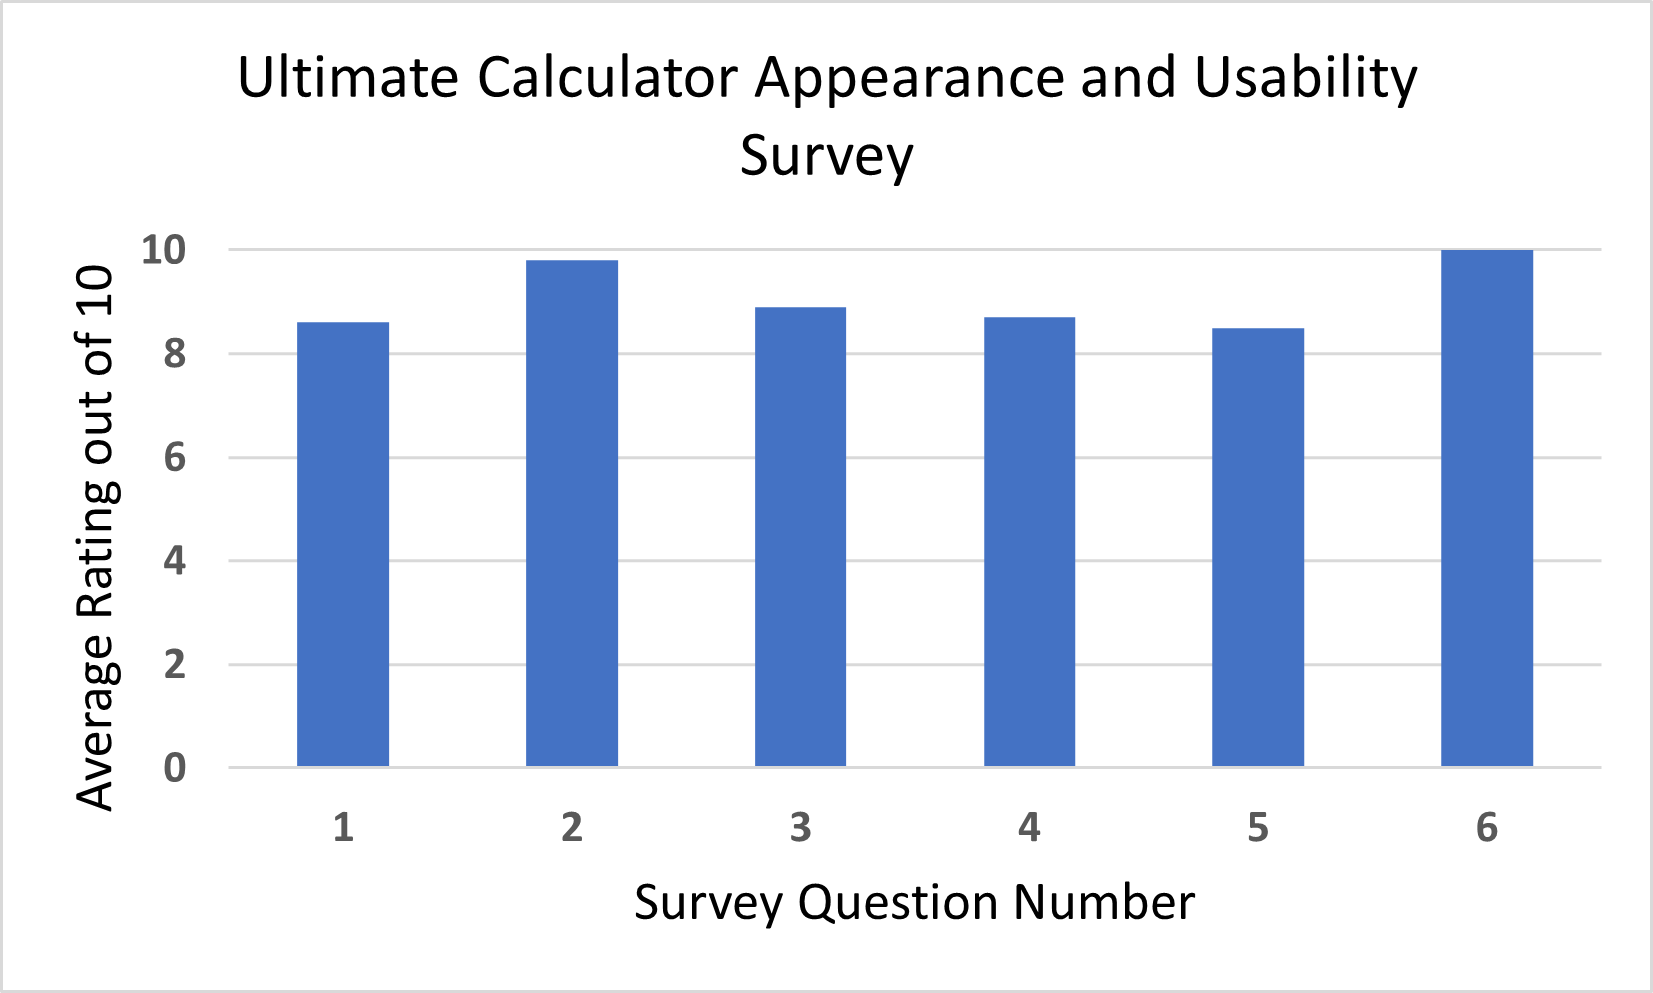
\includegraphics[scale=0.9]{surveyResults.png}
    \caption{Survey Results}
    \label{calc}
\end{figure}

As you can see, the overall results of the survey were very positive. They helped to aid in completing our tests for our non-functional requirements.
	
\section{Comparison to Existing Implementation}	

In the original source code of the Ultimate Calculator, there were no test cases that were implemented. In the updated version of Ultimate calculator, the source code was designed to be more modular than the original. The various calculator functionalities were split into their respective modules and unit testing was done to ensure accurate calculation results. The development team created documentation including a software requirements specification, test plan document and design documentation to organize the information via traceability of the requirements and the modules. The documentation also helps to catalog the test cases. The functional requirements were met through various testing methods such as unit testing and visual testing and there were a total of 110 unit test cases prior to the final demonstration of the project. 

\section{Unit Testing}
Unit testing was done for each module that contained the calculators functionality. These modules are found in the calculators file in the projects repository. These files provide the functionality to each module in the application. Using the unittest library, each tester created a unit test file for the modules they were responsible for creating and maintaining. At a minimum basic units tests were created for each function, along with tests that made sure the error handling for each function worked correctly.

\section{Changes Due to Testing}

The unit tests and manual tests were helpful in finding small oversights that we were unaware of. Some errors we found include numbers being too large to be displayed in the output text boxes, users being able to enter an infinite amount of characters which could break the application, and a handful of other errors. All these errors were fixed in the application following their discovery. Testing did not really change the requirements but was quite helpful in finding errors we didn't consider.

\section{Automated Testing}
Automated testing was used for the calculation portion of the calculator application. A unit testing module was created for each calculation module and every method was thoroughly tested to ensure accurate calculator results. The python unittest framework was used to test various calculation method outputs to ensure they met the threshold of a correct output.
\section{Trace to Requirements}
\begin{landscape}

\begin{table}[H]
\begin{center}
\caption{\textbf{Traceability Matrix for Calculation Requirements}} \label{trace3}
\begin{tabularx}{\textwidth}{cc|c|c|c|c|c|c|c|c|c|c|c|c|c|}
\cline{3-12}
& & \multicolumn{10}{ c|}{Requirements} \\ \cline{3-12}
& & FR1  & FR2 & FR3 & FR4 & FR5 & FR6 & FR7 & FR8 & FR9 & FR10  \\ \cline{1-12}
    \multicolumn{1}{ |c| }{\multirow{3}{*}{Test Cases} } &
    \multicolumn{1}{|c| } {FR-C-T1} &&&&&&X&X&&&\\ \cline{2-12}
        \multicolumn{1}{|c| }{} 	                  &
    \multicolumn{1}{|c| }{FR-C-T2} &&&&&&&&&&  \\ \cline{2-12}
    \multicolumn{1}{|c| }{} 	                  &
    \multicolumn{1}{|c| }{FR-C-T3} &&&&&&&&&& \\ \cline{2-12}
\end{tabularx}
\end{center}
\end{table}

\begin{table}[H]
\begin{center}
\caption{\textbf{Traceability Matrix for Calculation Requirements Continued}} \label{trace3}
\begin{tabularx}{\textwidth}{cc|c|c|c|c|c|c|c|c|c|c|c|c|c|c|}
\cline{3-13}
& & \multicolumn{11}{ c|}{Requirements} \\ \cline{3-13}
& & FR11  & FR12 & FR13 & FR14 & FR15 & FR16 & FR17 & FR18 & FR19 & FR20 & FR21  \\ \cline{1-13}
    \multicolumn{1}{ |c| }{\multirow{3}{*}{Test Cases} } &
    \multicolumn{1}{|c| } {FR-C-T1} &&&&&&&&&&&\\ \cline{2-13}
        \multicolumn{1}{|c| }{} 	                  &
    \multicolumn{1}{|c| }{FR-C-T2} &X&&&&&&&&&&  \\ \cline{2-13}
    \multicolumn{1}{|c| }{} 	                  &
    \multicolumn{1}{|c| }{FR-C-T3} &&&&X&&&&&&& \\ \cline{2-13}
\end{tabularx}
\end{center}
\end{table}

\newpage

\begin{table}[H]
\begin{center}
\caption{\textbf{Traceability Matrix for UI Requirements}} \label{trace3}
\begin{tabularx}{\textwidth}{cc|c|c|c|c|c|c|c|c|c|c|c|c|c|}
\cline{3-12}
& & \multicolumn{10}{ c|}{Requirements} \\ \cline{3-12}
& & FR1  & FR2 & FR3 & FR4 & FR5 & FR6 & FR7 & FR8 & FR9 & FR10  \\ \cline{1-12}
    \multicolumn{1}{ |c| }{\multirow{10}{*}{Test Cases} } &
    \multicolumn{1}{|c| } {FR-UI-T1} &X&&&X&&&&&&\\ \cline{2-12}
        \multicolumn{1}{|c| }{} 	                  &
    \multicolumn{1}{|c| }{FR-UI-T2} &&X&&&&&&&&  \\ \cline{2-12}
    \multicolumn{1}{|c| }{} 	                  &
    \multicolumn{1}{|c| }{FR-UI-T3} &&&X&&X&&&&& \\ \cline{2-12}
    \multicolumn{1}{|c| }{} 	                  &
    \multicolumn{1}{|c| }{FR-UI-T4} &&&&&&&&X&X&X \\ \cline{2-12}
    \multicolumn{1}{|c| }{}                        &
    \multicolumn{1}{|c| } {FR-UI-T5} &&&&&&&&&& \\ \cline{2-12}
    \multicolumn{1}{|c| }{} 	                  &
    \multicolumn{1}{|c| }{FR-UI-T6} &&&&&&&&&& \\ \cline{2-12}
    \multicolumn{1}{|c| }{} 	                  &
    \multicolumn{1}{|c| }{FR-UI-T7} &&&&&&&&&&  \\ \cline{2-12}
    \multicolumn{1}{|c| }{}                        &
    \multicolumn{1}{ |c| } {FR-UI-T8} &&&&&&&&&& \\ \cline{2-12}
    \multicolumn{1}{|c| }{}                        &
    \multicolumn{1}{ |c| } {FR-UI-T9} &&&&&&&&&& \\ \cline{2-12}
    \multicolumn{1}{|c| }{}                        &
    \multicolumn{1}{ |c| }{FR-UI-T10} &&&&&&&&&& \\ \cline{2-12}
\end{tabularx}
\end{center}
\end{table}

\begin{table}[H]
\begin{center}
\caption{\textbf{Traceability Matrix for UI Requirements Continued}} \label{trace3}
\begin{tabularx}{\textwidth}{cc|c|c|c|c|c|c|c|c|c|c|c|c|c|c|}
\cline{3-13}
& & \multicolumn{11}{ c|}{Requirements} \\ \cline{3-13}
& & FR11  & FR12 & FR13 & FR14 & FR15 & FR16 & FR17 & FR18 & FR19 & FR20 & FR21  \\ \cline{1-13}
    \multicolumn{1}{ |c| }{\multirow{10}{*}{Test Cases} } &
    \multicolumn{1}{|c| } {FR-UI-T1} &&&&&&&&&&&\\ \cline{2-13}
        \multicolumn{1}{|c| }{} 	                  &
    \multicolumn{1}{|c| }{FR-UI-T2} &&&&&&&&&&&  \\ \cline{2-13}
    \multicolumn{1}{|c| }{} 	                  &
    \multicolumn{1}{|c| }{FR-UI-T3} &&&&&&&&&&& \\ \cline{2-13}
    \multicolumn{1}{|c| }{} 	                  &
    \multicolumn{1}{|c| }{FR-UI-T4} &&&&&&&&&&& \\ \cline{2-13}
    \multicolumn{1}{|c| }{}                        &
    \multicolumn{1}{|c| } {FR-UI-T5} &&X&&&&&&&&& \\ \cline{2-13}
    \multicolumn{1}{|c| }{} 	                  &
    \multicolumn{1}{|c| }{FR-UI-T6} &&&X&&&&&&&& \\ \cline{2-13}
    \multicolumn{1}{|c| }{} 	                  &
    \multicolumn{1}{|c| }{FR-UI-T7} &&&&&X&&&&&&  \\ \cline{2-13}
    \multicolumn{1}{|c| }{}                        &
    \multicolumn{1}{ |c| } {FR-UI-T8} &&&&&&X&X&&&& \\ \cline{2-13}
    \multicolumn{1}{|c| }{}                        &
    \multicolumn{1}{ |c| } {FR-UI-T9} &&&&&&&&X&&& \\ \cline{2-13}
    \multicolumn{1}{|c| }{}                        &
    \multicolumn{1}{ |c| }{FR-UI-T10} &&&&&&&&&X&X&X \\ \cline{2-13}
\end{tabularx}
\end{center}
\end{table}

\newpage

\begin{table}[H]
\begin{center}
\caption{\textbf{Traceability Matrix for Non-Functional Requirements}} \label{trace3}
\begin{tabularx}{\textwidth}{cc|c|c|c|c|c|c|c|c|c|c|c|c|c|}
\cline{3-12}
& & \multicolumn{10}{ c|}{Requirements} \\ \cline{3-12}
& & NFR1  & NFR2 & NFR3 & NFR4 & NFR5 & NFR6 & NFR7 & NFR8 & NFR9 & NFR10  \\ \cline{1-12}
    \multicolumn{1}{ |c| }{\multirow{10}{*}{Test Cases} } &
    \multicolumn{1}{|c| } {NFR-LF-T1} &X&&&&&&&&&\\ \cline{2-12}
        \multicolumn{1}{|c| }{} 	                  &
    \multicolumn{1}{|c| }{NFR-LF-T2} &&X&&&&&&&&  \\ \cline{2-12}
    \multicolumn{1}{|c| }{} 	                  &
    \multicolumn{1}{|c| }{NFR-U-T1} &&&X&&&&&&& \\ \cline{2-12}
    \multicolumn{1}{|c| }{} 	                  &
    \multicolumn{1}{|c| }{NFR-U-T2} &&&&X&&&&&& \\ \cline{2-12}
    \multicolumn{1}{|c| }{}                        &
    \multicolumn{1}{|c| } {NFR-P-T1} &&&&&X&&&&& \\ \cline{2-12}
    \multicolumn{1}{|c| }{} 	                  &
    \multicolumn{1}{|c| }{NFR-P-T2} &&&&&&X&&&& \\ \cline{2-12}
    \multicolumn{1}{|c| }{} 	                  &
    \multicolumn{1}{|c| }{NFR-P-T3} &&&&&&&X&&&  \\ \cline{2-12}
    \multicolumn{1}{|c| }{}                        &
    \multicolumn{1}{ |c| } {NFR-OE-T1} &&&&&&&&X&& \\ \cline{2-12}
    \multicolumn{1}{|c| }{}                        &
    \multicolumn{1}{ |c| } {NFR-MS-T1} &&&&&&&&&X& \\ \cline{2-12}
    \multicolumn{1}{|c| }{}                        &
    \multicolumn{1}{ |c| }{NFR-MS-T2} &&&&&&&&&&X \\ \cline{2-12}
\end{tabularx}
\end{center}
\end{table}
\end{landscape}

\newpage		
\section{Trace to Modules}		
% the table should use mref, the requirements should be named, use something
% like fref
\begin{table}[H]
\centering
\begin{tabular}{p{0.2\textwidth} p{0.6\textwidth}}
\toprule
\textbf{Req.} & \textbf{Modules}\\
\midrule
FR1 & \hyperref[m1]{M1}\\
FR2 & \hyperref[m1]{M1}\\ 
FR3 & \hyperref[m5]{M5}, \hyperref[m6]{M6}, \hyperref[m7]{M7}, \hyperref[m10]{M10}, \hyperref[m11]{M11}, \hyperref[m14]{M14}, \hyperref[m15]{M15}, \hyperref[m16]{M16}, \hyperref[m17]{M17}, \hyperref[m20]{M20}, \hyperref[m21]{M21}, \hyperref[m22]{M22}, \hyperref[m25]{M25}, \hyperref[m26]{M26}, \hyperref[m27]{M27}, \hyperref[m28]{M28}, \hyperref[m30]{M30} \\
FR4 & \hyperref[m1]{M1}\\
FR5 & \hyperref[m3]{M3}, \hyperref[m5]{M5}, \hyperref[m6]{M6}, \hyperref[m7]{M7}, \hyperref[m8]{M8}, \hyperref[m10]{M10}, \hyperref[m11]{M11}, \hyperref[m12]{M12}, \hyperref[m14]{M14}, \hyperref[m15]{M15}, \hyperref[m16]{M16}, \hyperref[m17]{M17}, \hyperref[m18]{M18}, \hyperref[m20]{M20}, \hyperref[m21]{M21}, \hyperref[m22]{M22}, \hyperref[m23]{M23}, \hyperref[m25]{M25}, \hyperref[m26]{M26}, \hyperref[m27]{M27}, \hyperref[m28]{M28}, \hyperref[m30]{M30}\\
FR6 & \hyperref[m5]{M5}, \hyperref[m6]{M6}, \hyperref[m7]{M7}, \hyperref[m10]{M10}, \hyperref[m11]{M11}, \hyperref[m14]{M14}, \hyperref[m15]{M15}, \hyperref[m16]{M16}, \hyperref[m17]{M17}, \hyperref[m20]{M20}, \hyperref[m21]{M21}, \hyperref[m22]{M22}, \hyperref[m25]{M25}, \hyperref[m26]{M26}, \hyperref[m27]{M27}, \hyperref[m28]{M28}, \hyperref[m30]{M30}\\
FR7 & \hyperref[m5]{M5}, \hyperref[m6]{M6}, \hyperref[m7]{M7}, \hyperref[m10]{M10}, \hyperref[m11]{M11}, \hyperref[m14]{M14}, \hyperref[m15]{M15}, \hyperref[m16]{M16}, \hyperref[m17]{M17}, \hyperref[m20]{M20}, \hyperref[m21]{M21}, \hyperref[m22]{M22}, \hyperref[m25]{M25}, \hyperref[m26]{M26}, \hyperref[m27]{M27}, \hyperref[m28]{M28}, \hyperref[m30]{M30}\\
FR8 & \hyperref[m5]{M5}, \hyperref[m6]{M6}, \hyperref[m7]{M7}, \hyperref[m10]{M10}, \hyperref[m11]{M11}, \hyperref[m14]{M14}, \hyperref[m15]{M15}, \hyperref[m16]{M16}, \hyperref[m17]{M17}, \hyperref[m20]{M20}, \hyperref[m21]{M21}, \hyperref[m22]{M22}, \hyperref[m25]{M25}, \hyperref[m26]{M26}, \hyperref[m27]{M27}, \hyperref[m28]{M28}, \hyperref[m30]{M30}\\
FR9 & \hyperref[m5]{M5}, \hyperref[m6]{M6}, \hyperref[m7]{M7}, \hyperref[m10]{M10}, \hyperref[m11]{M11}, \hyperref[m14]{M14}, \hyperref[m15]{M15}, \hyperref[m16]{M16}, \hyperref[m17]{M17}, \hyperref[m20]{M20}, \hyperref[m21]{M21}, \hyperref[m22]{M22}, \hyperref[m25]{M25}, \hyperref[m26]{M26}, \hyperref[m27]{M27}, \hyperref[m28]{M28}, \hyperref[m30]{M30}\\
FR10 & \hyperref[m5]{M5}, \hyperref[m6]{M6}, \hyperref[m7]{M7}, \hyperref[m10]{M10}, \hyperref[m11]{M11}, \hyperref[m14]{M14}, \hyperref[m15]{M15}, \hyperref[m16]{M16}, \hyperref[m17]{M17}, \hyperref[m20]{M20}, \hyperref[m21]{M21}, \hyperref[m22]{M22}, \hyperref[m25]{M25}, \hyperref[m26]{M26}, \hyperref[m27]{M27}, \hyperref[m28]{M28}, \hyperref[m30]{M30}\\
FR11 & \hyperref[m5]{M5}, \hyperref[m6]{M6}, \hyperref[m7]{M7}, \hyperref[m10]{M10}, \hyperref[m11]{M11}, \hyperref[m14]{M14}, \hyperref[m15]{M15}, \hyperref[m16]{M16}, \hyperref[m17]{M17}, \hyperref[m20]{M20}, \hyperref[m21]{M21}, \hyperref[m22]{M22}, \hyperref[m25]{M25}, \hyperref[m26]{M26}, \hyperref[m27]{M27}, \hyperref[m28]{M28}, \hyperref[m30]{M30}\\
FR12 & \hyperref[m5]{M5}, \hyperref[m6]{M6}, \hyperref[m7]{M7}, \hyperref[m10]{M10}, \hyperref[m11]{M11}, \hyperref[m14]{M14}, \hyperref[m15]{M15}, \hyperref[m16]{M16}, \hyperref[m17]{M17}, \hyperref[m20]{M20}, \hyperref[m21]{M21}, \hyperref[m22]{M22}, \hyperref[m25]{M25}, \hyperref[m26]{M26}, \hyperref[m27]{M27}, \hyperref[m28]{M28}, \hyperref[m30]{M30}\\
FR13 & \hyperref[m5]{M5}, \hyperref[m6]{M6}, \hyperref[m7]{M7}, \hyperref[m10]{M10}, \hyperref[m11]{M11}, \hyperref[m14]{M14}, \hyperref[m15]{M15}, \hyperref[m16]{M16}, \hyperref[m17]{M17}, \hyperref[m20]{M20}, \hyperref[m21]{M21}, \hyperref[m22]{M22}, \hyperref[m25]{M25}, \hyperref[m26]{M26}, \hyperref[m27]{M27}, \hyperref[m28]{M28}, \hyperref[m30]{M30}\\
FR14 & \hyperref[m2]{M2}, \hyperref[m4]{M4}, \hyperref[m9]{M9}, \hyperref[m13]{M13}, \hyperref[m19]{M19}, \hyperref[m24]{M24}, \hyperref[m29]{M29}, \hyperref[m31]{M31}\\
FR15 & \hyperref[m5]{M5}, \hyperref[m6]{M6}, \hyperref[m7]{M7}, \hyperref[m10]{M10}, \hyperref[m11]{M11}, \hyperref[m14]{M14}, \hyperref[m15]{M15}, \hyperref[m16]{M16}, \hyperref[m17]{M17}, \hyperref[m20]{M20}, \hyperref[m21]{M21}, \hyperref[m22]{M22}, \hyperref[m25]{M25}, \hyperref[m26]{M26}, \hyperref[m27]{M27}, \hyperref[m28]{M28}, \hyperref[m30]{M30}\\
FR16 & \hyperref[m5]{M5}, \hyperref[m6]{M6}, \hyperref[m7]{M7}, \hyperref[m10]{M10}, \hyperref[m11]{M11}, \hyperref[m14]{M14}, \hyperref[m15]{M15}, \hyperref[m16]{M16}, \hyperref[m17]{M17}, \hyperref[m20]{M20}, \hyperref[m21]{M21}, \hyperref[m22]{M22}, \hyperref[m25]{M25}, \hyperref[m26]{M26}, \hyperref[m27]{M27}, \hyperref[m28]{M28}, \hyperref[m30]{M30}\\
FR17 & \hyperref[m5]{M5}, \hyperref[m6]{M6}, \hyperref[m7]{M7}, \hyperref[m10]{M10}, \hyperref[m11]{M11}, \hyperref[m14]{M14}, \hyperref[m15]{M15}, \hyperref[m16]{M16}, \hyperref[m17]{M17}, \hyperref[m20]{M20}, \hyperref[m21]{M21}, \hyperref[m22]{M22}, \hyperref[m25]{M25}, \hyperref[m26]{M26}, \hyperref[m27]{M27}, \hyperref[m28]{M28}, \hyperref[m30]{M30}\\
FR18 & \hyperref[m5]{M5}, \hyperref[m6]{M6}, \hyperref[m7]{M7}, \hyperref[m10]{M10}, \hyperref[m11]{M11}, \hyperref[m14]{M14}, \hyperref[m15]{M15}, \hyperref[m16]{M16}, \hyperref[m17]{M17}, \hyperref[m20]{M20}, \hyperref[m21]{M21}, \hyperref[m22]{M22}, \hyperref[m25]{M25}, \hyperref[m26]{M26}, \hyperref[m27]{M27}, \hyperref[m28]{M28}, \hyperref[m30]{M30}\\
FR19 & \hyperref[m1]{M1}\\
FR20 & \hyperref[m1]{M1}, \hyperref[m3]{M3}, \hyperref[m5]{M5}, \hyperref[m6]{M6}, \hyperref[m7]{M7}, \hyperref[m8]{M8}, \hyperref[m10]{M10}, \hyperref[m11]{M11}, \hyperref[m12]{M12}, \hyperref[m14]{M14}, \hyperref[m15]{M15}, \hyperref[m16]{M16}, \hyperref[m17]{M17}, \hyperref[m18]{M18}, \hyperref[m20]{M20}, \hyperref[m21]{M21}, \hyperref[m22]{M22}, \hyperref[m23]{M23}, \hyperref[m25]{M25}, \hyperref[m26]{M26}, \hyperref[m27]{M27}, \hyperref[m28]{M28}, \hyperref[m30]{M30}\\
FR21 & \hyperref[m1]{M1}\\
\bottomrule
\end{tabular}
\caption{Trace Between Requirements and Modules}
\label{TblRT}
\end{table}
\section{Code Coverage Metrics}
In the test plan, our goal was to have a STATEMENT\_COV \% statement coverage in regards to any modules in which unit testing is applicable. Through the use of a tool known as Coverage.py, we found these results:
\begin{enumerate}
    \item Statement coverage of algebra\_calculator.py: 94\%
    \item Statement coverage of binary\_calculator.py: 99\%
    \item Statement coverage of conversion\_calculator.py: 96\%
    \item Statement coverage of geometry\_calculator.py: 95\%
    \item Statement coverage of gpa\_calculator.py: 100\%
    \item Statement coverage of health\_calculator.py: 100\%
    \item Statement coverage of main\_calculator.py: 95\%
    \item Statement coverage of stocks\_calculator.py: 100\%
\end{enumerate}

As you can see from the results we gathered, we well surpassed our goals for statement coverage with unit testing.

\section{Appendix}

%This is where you can place additional information.

\subsection{Symbolic Parameters}
\label{sec:sp}

SURVEY\_SCORE = 80\\
STATEMENT\_COV = 80\\
MAX\_RESPONSE\_TIME = 2\\
MAX\_NAVIGATION\_CLICKS = 2\\
MAX\_SIG\_FIGS = 64\\
MIN\_UNIQUE\_OP = 5\\
MIN\_OP\_SECTION = \textcolor{Green}{1}\\
MIN\_INPUT = 1\\

\subsection{Usability Survey Questions}
\label{sec:survey}

\textbf{All questions will be answered on a 1-10 scale}

\begin{enumerate}

\item How familiar does the main menu screen feel to a standard calculator?
    
\item How cohesive do the styles of each window (colours, button sizes, input methods, etc.) feel to one another?

\item Starting from the main menu, try navigating to the Temperature Converter operation. How easy was it to locate said operation?

\item How intuitive does the navigation between different sections of the calculator feel?

\item How fluid do the transitions between different operations of calculator feel?

\item How timely do the answers received from calculations feel? 

\end{enumerate}


\subsection{Generic Calculator for Comparison}

\begin{figure}[H]
    \centering
    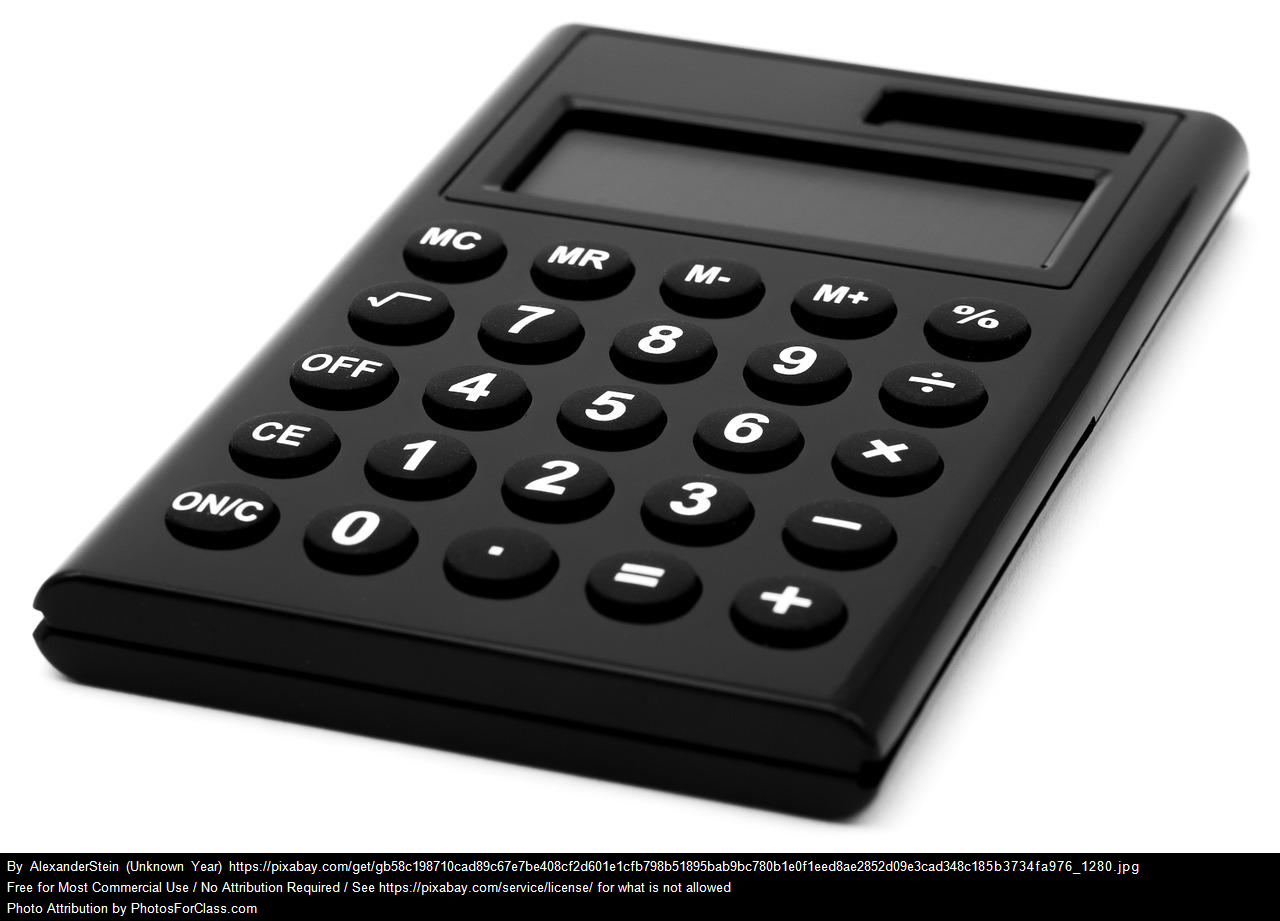
\includegraphics[scale=0.4]{Calc.png}
    \caption{Generic Calculator}
    \label{calc}
\end{figure}

\bibliographystyle{plainnat}

\bibliography{SRS}

\end{document}